\section{Experiments}
Here follow some of the experiments conducted throughout the thesis. All of them were run on a Python-based algorithm, on a computer with an AMD Ryzen 7 4800H octa-core processor, running at 2900 MHz, and 16GB of RAM. Analysis of the results is done more in-depth under section 5.

\subsection{Exhaustive Vertex-Based Graph Generation}
This plot represents the time taken to generate (and analyze) all the graphs, according to their number of vertices, following CGE's brute-force approach.
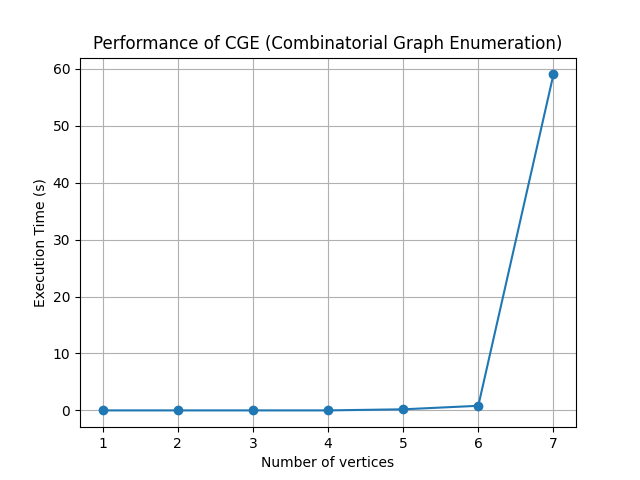
\includegraphics[width=7.5cm]{images/cge_testing.png}

\subsection{Erdős–Rényi Binomial Graph Generation}
This plot represents the time taken to generate (and analyze) 10,000 graphs with a 50\% probability of creating an edge between any two vertices, according to their number of vertices, following the random sampling approach. The impact of the exponentiality on the CPU time is clearly noticeable after a certain number of vertices, both for this and the previous plots. 
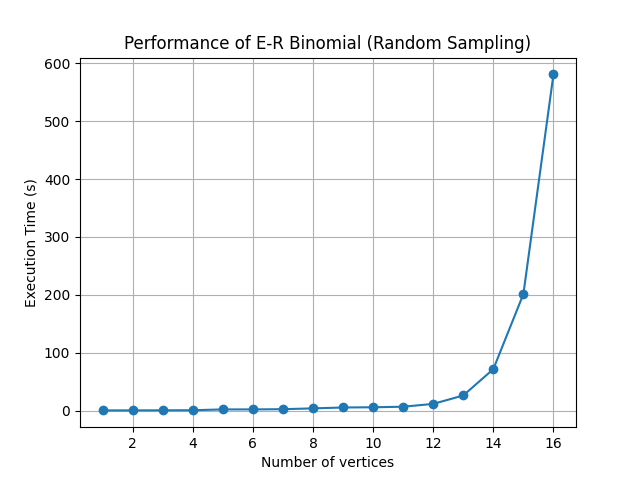
\includegraphics[width=7.5cm]{images/rnd_testing_16.png}

\subsubsection{Linear Regression Model for Highest Treewidth Ratios}
This plot represents the results of looking for the optimization values of the parameters that are relevant in the random sampling. The model was developed for $F(k)$, where $k=4$. The step size used was 0.25 on the different edge probabilities that were being tested, and the one that yielded the highest correct treewidth ratio was kept. The optimization process was performed on $n=10,000$.

In other words, the goal of this model is to maximize the number of relevant graphs that are randomly generated by the Erdős–Rényi approach. It is a method of pruning the search space, inherently considering the optimal edge probabilities that, given any sample, generate graphs whose treewidth is $k+1$, to begin with. Therefore, the base sample is being optimized to provide the highest chances of finding a minimal forbidden minor, according to the number of vertices. 

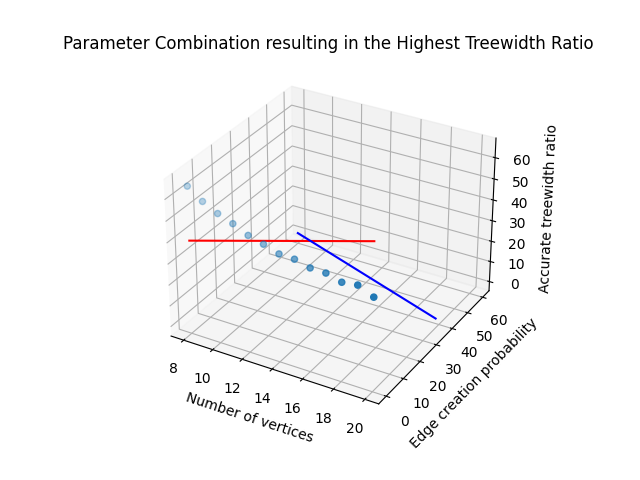
\includegraphics[width=7.5cm]{images/tw_ratio_3d.png}
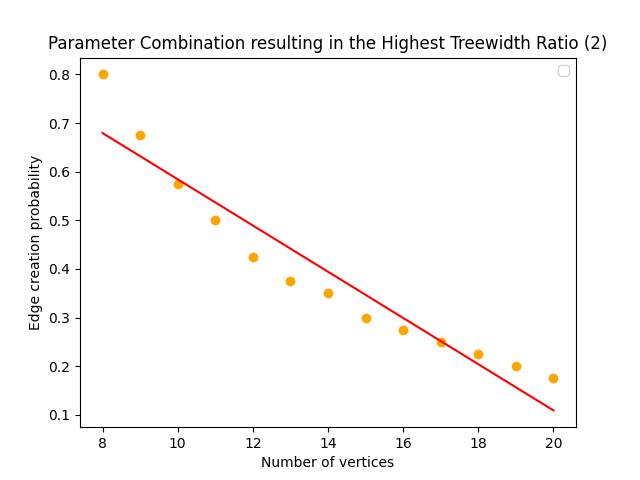
\includegraphics[width=3.75cm]{images/tw_ratio_2d_edge.png}
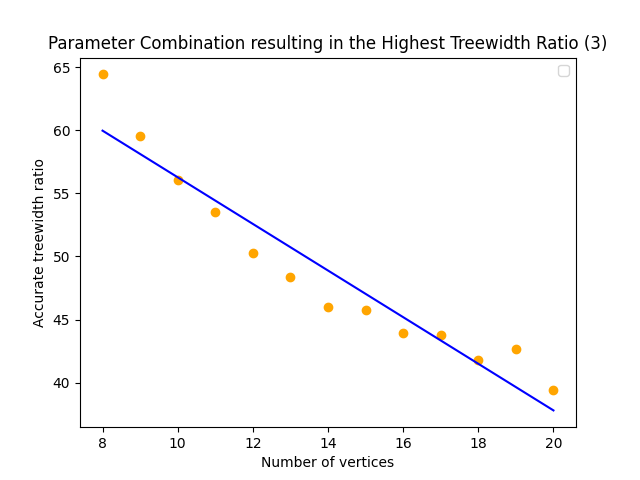
\includegraphics[width=3.75cm]{images/tw_ratio_2d_tw.png}

The bottom two plots show the optimal values for edge creation (left) that result in the corresponding highest accurate treewidth ratios (right) generated as a consequence of those optimal values. The top plot is a 3-dimensional visualization of the same parameters. The trend is thus: the lower the number of vertices, the higher the edge creation probability that achieves the highest ratio of graphs with the desired treewidth. As a rule of thumb, if the edge probability is too high, graphs with treewidth strictly higher than $k+1$ will be found; and if it is too low, graphs with treewidth strictly lower than that will be found. Neither of which fit the purposes of the process.

\subsubsection{Average Number of Runs until the Finding of an MFM}
This plot shows the average number of iterations that the program runs until a minimal forbidden minor is found, within the binomial random sampling approach. Note that this does not account for new minors, it solely represents the frequency of minors, many of which are isomorphic with other found minimal forbidden minors. The optimal binomial parameters for $k=4$ (plotted in the previous experiment) were used to compute this data.

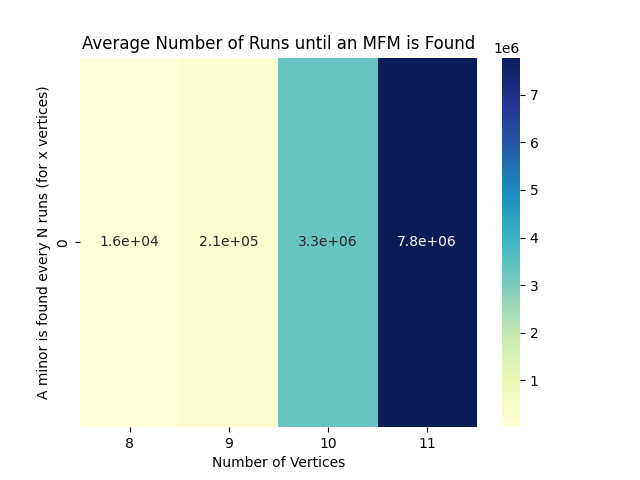
\includegraphics[width=7.5cm]{images/avg_runs_until_minor.png}

\subsubsection{Binomial Sampling Coverage}
This plot demonstrates how the size of the sample that is feasible to generate compares with the number of non-isomorphic connected graphs existent in the space, according to their number of vertices \cite{oeisA001349}.

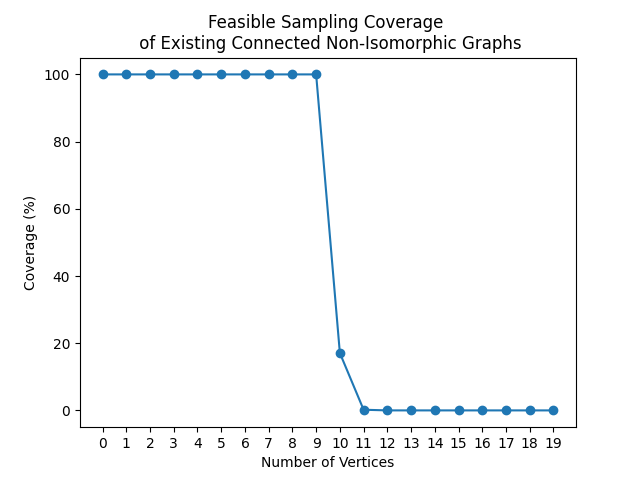
\includegraphics[width=7.5cm]{images/sampling_cover.png}

\subsection{How does Pre-MFM-Finding Connectivity Checking improve Performance?}
This shows the search space pruning that is achievable by performing a connectivity check before analyzing the generated graph datasets.

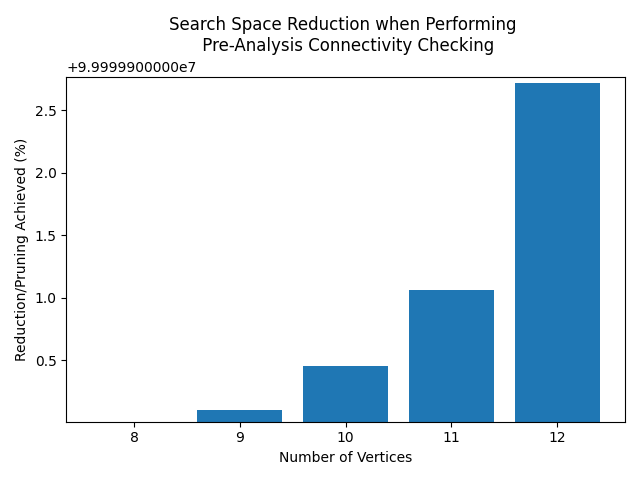
\includegraphics[width=6.5cm]{images/conn_pruning.png}

\subsection{Performing MFM-Finding Analysis at every condition (AEC) vs. at basic structure (ABS) alone}
This experiment studies the impact of analyzing the generated graphs solely in their original generated format/structure versus at also every graph deconstruction, i.e. at every vertex deletion and at every edge deletion or contraction. It ran on a set of 50,000 generated graphs, with optimal treewidth ratio parameters for 9 vertices (from 3.2.1). It is possible to see the computational time and the practical outcome performance.

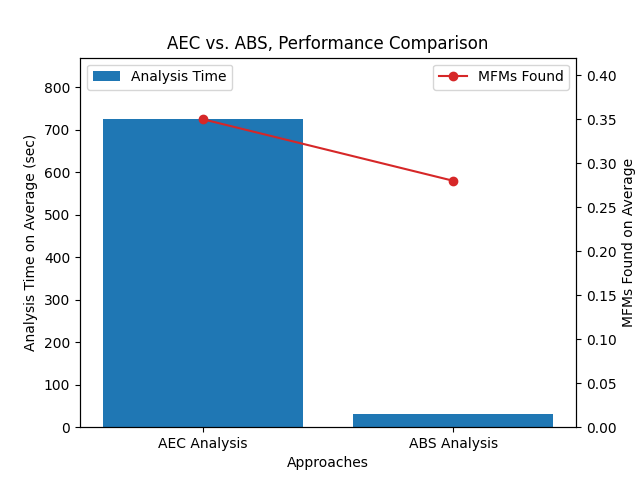
\includegraphics[width=7.5cm]{images/aec_vs_abs.png}


